\section{3-Dimensional Space}

The 3-D coordinate system is often denoted by $\R^3$. Likewise, the 2-D coordinate system is denoted by $\R^2$, and the 1-D coordinate system is denoted by $\R$.

%%%%%%%%%%%%%%%%%%%%%%%%
%  Equations of Lines  %
%%%%%%%%%%%%%%%%%%%%%%%%

\subsection{Equations of Lines}

\Note[Vector form]{
    If $\vec{a}$ and $\vec{v}$ are parallel vectors, then $\vec{a} = t \vec{v}$ for some scalar $t$. \\
    Now if we have a vector $\vec{r}$ as follows \[ 
        \vec{r} = \vec{r_0} + \vec{a}
    \]
    Then we can write \[ 
        \vec{r} = \vec{r_0} + t \vec{v} = \langle x_0,y_0,z_0 \rangle + t \langle a,b,c \rangle
    \]
    This is called the \textbf{vector form of the equation of a line}.
}

\Note[Parametric form]{
    We can rewrite the vector form as
    \begin{align*}
        \vec{r} &= \langle x_0,y_0,z_0 \rangle + t \langle a,b,c \rangle \\
        \langle x,y,z \rangle &= \langle x_0+ta, y_0+tb, z_0+tc \rangle
    \end{align*}
    In other words
    \begin{align*}
        x &= x_0 + ta \\
        y &= y_0 + tb \\ 
        z &= z_0 + tc
    \end{align*}
    This set of equations is called the \textbf{parametric form of the equation of a line}.
}

\Note[Symmetric Equations of a Line]{
    If we assume that $a, b$, and $c$ are non-zero numbers, then we can solve each of the parametric equations for $t$. This gives us \[ 
        \frac{x-x_0}{a} = \frac{y-y_0}{b} = \frac{z-z_0}{c}
    \]
}

\Example{Find the Equations of lines: \\
    \textbf{1.} Through the points $(7,-3,1)$ and $(-2,1,4)$ \\
    \textbf{2.} Through the point $(1,-5,0)$ and parallel to the line given by $\vec{r}(t) = \langle 8-3t, -10+9t, -1-t \rangle$ \\
    \textbf{3.} Through the point $(-7,2,4)$ and orthogonal to both $\vec{v}=\langle 0,-9,1 \rangle$ and $\vec{w}=3 \hat{i} + \hat{j} - 4 \hat{k}$ \\
}{
    \textbf{1.} \\
        Direction vector $\vec{d} = \langle -2-7, 1+3, 4-1 \rangle = \langle -9,4,3 \rangle$ \\
        Now, the vector form of the line is \[ 
            \vec{r} = \langle 7,-3,1 \rangle + t \langle -9,4,3 \rangle
        \]
        The parametric form is \[ 
            x = 7 - 9t, \quad y = -3 + 4t, \quad z = 1 + 3t
        \]
        The symmetric form is \[ 
            \frac{x-7}{-9} = \frac{y+3}{4} = \frac{z-1}{3}
        \]
    \textbf{2.} \\
        The direction vector is $\vec{d} = \langle -3, 9, -1 \rangle$ \\ 
        Hence, the vector form of the line is \[ 
            \vec{r} = \langle 1,-5,0 \rangle + t \langle -3,9,-1 \rangle 
        \]
        The parametric form is \[ 
            x = 1 + 3t, \quad y = -5 + 9t, \quad z = -t 
        \]
        And the symmetric form is \[ 
            \frac{x-1}{3} = \frac{y+5}{9} = -z 
        \]
    \textbf{3.} \\ 
    Direction vector \[
        \vec{d} = \vec{v} \times \vec{w} 
        = \begin{vmatrix}
            \hat{i} & \hat{j} & \hat{k} \\
            0 & -9 & 1 \\
            3 & 1 & -4
        \end{vmatrix}
        = \langle 35,3,27 \rangle
    \]
    Hence, the vector form of the line is \[ 
        \vec{r} = \langle -7,2,4 \rangle + t \langle 35,3,27 \rangle 
    \]
    The parametric form is \[ 
        x = -7 + 35t, \quad y = 2 + 3t, \quad z = 4 + 27t
    \]
    The symmetric form is \[ 
        \frac{x+7}{35} = \frac{y-2}{3} = \frac{z-4}{27}
    \]
}

\Example{Determine if the two lines are parallel, orthogonal, or neither: \\
\textbf{1.} The line given by $\vec{r}(t) = \langle 4-7t, -10+5t, 21-4t \rangle$ and the line given by $\vec{r}(t) = \langle -2+3t, 7+5t, 5+t \rangle$ \\ 
\textbf{2.} The line given by $x=29, y=-3-6t, z=12-t$ and the line given by $\vec{r}(t) = \langle 12-14t, 2+7t, -10+3t \rangle$
}{
    \textbf{1.} \\ 
    The direction vectors are \[ 
        \vec{d_1} = \langle -7,5,-4 \rangle, \quad \vec{d_2} = \langle 3,5,1 \rangle
    \]
    To check if they are parallel, we can check: \[ 
        \frac{-7}{3} \neq \frac{5}{5} \neq \frac{-4}{1}
    \]
    which means they are not parallel. \\
    To check if they are orthogonal, we can check: \[ 
        \vec{d_1} \cdot \vec{d_2} = -7(3) + 5(5) + (-4)(1) = -21 + 25 - 4 = 0 
    \]
    Hence, they are orthogonal. \\
    \textbf{2.} \\ 
    The direction vectors are \[ 
        \vec{d_1} = \langle 0,-6,-1 \rangle, \quad \vec{d_2} = \langle -14,7,3 \rangle 
    \]
    To check if they are parallel, we can check: \[ 
        \frac{0}{-14} \neq \frac{-6}{7} \neq \frac{-1}{3} 
    \]
    which means they are not parallel. \\ 
    To check if they are orthogonal, we can check: \[ 
        \vec{d_1} \cdot \vec{d_2} = 0(-14) + (-6)(7) + (-1)(3) = -42 - 3 = -45 \neq 0
    \]
    Hence, they are neither parallel nor orthogonal.
}

\Example{Determine the intersection point of the two lines or show that they don't not intersect: \\ 
\textbf{1.} The line passing through the point $(0,-9,-1)$ and $(1,6,-3)$ and the line given by $\vec{r}(t) = \langle -9-4t, 10+6t, 1-2t \rangle$ \\
\textbf{2.} The line given by $x=1+6t, y=-1-3t, z=4+12t$ and the line given by $x=4+t, y=-10-8t, z=3-5t$
}{
    \textbf{1.} \\ 
    The direction vector of the first line is \[ 
        \vec{d_1} = \langle 1-0, 6+9, -3+1 \rangle = \langle 1,15,-2 \rangle
    \]
    We can write the parametric equations of the first line as: \[ 
        x = s, y = -9 + 15s, z = -1 - 2s
    \]
    And the parametric equations of the second line as: \[ 
        x = -9 - 4t, y = 10 + 6t, z = 1 - 2t
    \]
    Setting them equal to each other we get,
    \begin{align*}
        0 + t &= -9 - 4s \\
        -9 + 15t &= 10 + 6s \\
        -1 - 2t &= 1 - 2s
    \end{align*}
    Solving the first two equations, we get \[ 
        t = -\frac{7}{3}, \quad s = \frac{1}{3}
    \]
    Now, verifying the third equation, we get
    \begin{align*}
        -1 - 2(-\frac{7}{3}) &= 1 - 2(\frac{1}{3}) \\
        -1 + \frac{14}{3} &= 1 - \frac{2}{3} \\
        \frac{11}{3} &\neq \frac{1}{3}
    \end{align*}
    Since the third equation is not satisfied, the two lines do not intersect. \\ 
    \textbf{2.} \\ 
    The lines are given in parametric form. \\ 
    Setting them equal to each other we get,
    \begin{align*}
        1 + 6s &= 4 + t \\
        -1 - 3s &= -10 - 8t \\
        4 + 12s &= 3 - 5t
    \end{align*}
    Solving the first two equations, we get \[ 
        s = \frac{1}{3}, \quad t = -1
    \]
    Now, verifying the third equation, we get
    \begin{align*}
        4 + 12 \left( \frac{1}{3} \right) &= 3 - 5 \langle -1 \rangle \\
        8 &= 8
    \end{align*}
    That means, the lines intersect. Substituting the values in the parametric equation, we get
    \begin{align*}
        x &= 1 + 6 \left( \frac{1}{3} \right) = 3 \\ 
        y &= -1 - 3 \left( \frac{1}{3} \right) = -2 \\ 
        z &= 4 + 12 \left( \frac{1}{3} \right) = 8 
    \end{align*}
    Hence, the intersection point is $(3,-2,8)$.
}

\Example{Which of the three coordinate planes does the line given by $x = 16t, y = -4-9t, z = 34$ intersect?}{
    To intersect the $xy$-plane, we need $z=0$. But here $z=34$ is constant. Hence, the line does not intersect the $xy$-plane. \\
    To intersect the $yz$-plane, we need $x=0$. Hence, \[ 
        16t = 0 \implies t = 0 
    \]
    And the intersection point is $\left( 0, -4 - 9\times0 , 34 \right)$ or $(0, -4, 34)$. \\
    To intersect the $xz$-plane, we need $y=0$. Hence, \[ 
        -4 - 9t = 0 \implies t = -\frac{4}{9}
    \]
    And the intersection point is $\left( 16 \left( -\frac{4}{9} \right), 0, 43 \right)$ or $\left( -\frac{64}{9}, 0, 34 \right)$. \\
}


%%%%%%%%%%%%%%%%%%%%%%%%%
%  Equations of Planes  %
%%%%%%%%%%%%%%%%%%%%%%%%%

\subsection{Equations of Planes}

\Note[Vector form]{
    Let's assume $\vec{r_0} = \langle x_0,y_0,z_0 \rangle$ and $\vec{r} = \langle x,y,z \rangle$ are two position vectors and $\vec{r} - \vec{r_0}$ is a vector in the plane. \\ 
    If $\vec{n} = \langle a,b,c \rangle$ is a normal to the plane (which means it's orthogonal to the vector $\vec{r} - \vec{r_0}$), then we can write \[ 
        \vec{n} \cdot (\vec{r} - \vec{r_0}) = 0 \quad\implies\quad \vec{n} \cdot \vec{r} = \vec{n} \cdot \vec{r_0}
    \]
    This is called the \textbf{vector form of the equation of a plane}.
}

\Note[Scalar form]{
    If we expand the vector equation in the following way,
    \begin{align*}
        \vec{n} \cdot (\vec{r} - \vec{r_0}) &= 0 \\ 
        \langle a,b,c \rangle \cdot \langle x-x_0, y-y_0, z-z_0 \rangle &= 0
    \end{align*}
    Computing the dot product, we get \[ 
        a(x-x_0) + b(y-y_0) + c(z-z_0) = 0
    \]
    This is called the \textbf{scalar form of the equation of a plane}. \\ 
    This equation can also be written as \[ 
        ax + by + cz = d
    \]
    where $d = ax_0 + by_0 + cz_0$.
}

\Example{Find the equation of the plane: \\
\textbf{1.} Through the point $(6,-3,1)$, $(5,-4,1)$, and $(3,-4,0)$ \\
\textbf{2.} The plane containing the point $(1,-5,8)$ and orthogonal to the line given by $x=-3+15t, y=14-t, z=9-3t$ \\
\textbf{3.} The plane containing the point $(-8,3,7)$ and parallel to the plane given by $4x+8y-2z=45$ \\
\textbf{4.} The plane containing the two lines given by $\vec{r}(t) = \langle 7+5t, 2+t, 6t \rangle$ and $\vec{r}(t) = \langle 7-6t, 2-2t, 10t \rangle$
}{
    \textbf{1.} \\ 
    The given points are \[ 
        A(6,-3,1), B(5,-4,1), C(3,-4,0)
    \]
    Two vectors in the plane are
    \begin{align*}
        \vec{AB} &= \langle 5-6, -4+3, 1-1 \rangle = \langle -1,-1,0 \rangle \\
        \vec{BC} &= \langle 3-5, -4+4, 0-1 \rangle = \langle -2,0,-1 \rangle
    \end{align*}
    Normal vector on the place: \[ 
        \vec{n} = \begin{vmatrix}
            \hat{i} & \hat{j} & \hat{k} \\
            -1 & -1 & 0 \\ 
            -2 & 0 & -1
        \end{vmatrix}
        = \hat{i} -\hat{j} - 2\hat{k}
    \]
    Now, using the point $A$, we can write the equation of the plane as
    \begin{align*}
        (x-6) - (y+3) - 2(z-1) &= 0 \\
        x - y - 2z &= 7
    \end{align*}
    \textbf{2.} \\
    The normal vector is \[ 
        \vec{n} = \langle 15, -1, -3 \rangle
    \]
    Using the point $(1,-5,8)$, the equation of the plane is
    \begin{align*}
        15(x-1) -(y+5) -3(z-8) &= 0 \\
        15x - y - 3z &= 15 + 5 - 24 \\
        15x - y - 3z + 4 &= 0
    \end{align*}
    \textbf{3.} \\ 
    The normal vector is \[ 
        \vec{n} = \langle 4,8,-2 \rangle
    \]
    Using the point $(-8,3,7)$, the equation of the plane is
    \begin{align*}
        4(x+8) + 8(y-3) -2(z-7) &= 0 \\
        4x + 8y - 2z &= -32 + 24 + 14 \\
        4x + 8y - 2z + 6 &= 0 
    \end{align*}
    \textbf{4.} \\ 
    The direction vectors of the two lines are \[ 
        \vec{d_1} = \langle 5,1,6 \rangle, \quad \vec{d_2} = \langle -6,-2,10 \rangle
    \]
    The normal vector is \[ 
        \vec{n} = \vec{d_1} \times \vec{d_2} = \begin{vmatrix}
            \hat{i} & \hat{j} & \hat{k} \\
            5 & 1 & 6 \\ 
            -6 & -2 & 10
        \end{vmatrix}
        = \langle 22, -86, -4 \rangle 
    \]
    Using the point $A(7,2,0)$, the equation of the plane is
    \begin{align*}
        22(x-7) -86(y-2) -4(z-0) &= 0 \\
        22x - 86y - 4z - 154 + 172 &= 0 \\ 
        22x - 86y - 4z + 18 &= 0
    \end{align*}
}

\Example{Determine if the two planes are parallel, orthogonal, or neither: \\
The plane given by $3x+9y+7z=-1$ and the plane containing the points $(1,-1,9), (4,-1,2), (-2,3,4)$
}{
    The normal vector of the first plane is \[ 
        \vec{n_1} = \langle 3,9,7 \rangle
    \]
    Let the points be \[ 
        A(1,-1,9), B(4,-1,2), C(-2,3,4)
    \]
    Two vectors in the plane are
    \begin{align*}
        \vec{AB} &= \langle 4-1, -1+1, 2-9 \rangle = \langle 3,0,-7 \rangle \\
        \vec{AC} &= \langle -2-1, 3+1, 4-9 \rangle = \langle -3,4,-5 \rangle
    \end{align*}
    The normal vector of the second plane is \[ 
        \vec{n_2} = \vec{AB} \times \vec{AC} = \begin{vmatrix}
            \hat{i} & \hat{j} & \hat{k} \\
            3 & 0 & -7 \\ 
            -3 & 4 & -5
        \end{vmatrix}
        = \langle 28, 36, 12 \rangle = \langle 7,9,3 \rangle
    \]
    To check if they are parallel, we can check: \[ 
        \frac{3}{7} \neq \frac{9}{9} \neq \frac{7}{3}
    \]
    which means they are not parallel. \\ 
    To check if they are orthogonal, we can check: \[ 
        \vec{n_1} \cdot \vec{n_2} = 3(7) + 9(9) + 7(3) = 21 + 81 + 21 = 123 \neq 0
    \]
    Hence, they are neither parallel nor orthogonal.
}

\Example{Find the intersection of the plane given by $4x+y+10z=-2$ and the plane given by $-8x+2y+3z=-8$}{
    The two planes are 
    \begin{align*}
        4x + y + 10z &= -2 \\
        -8x + 2y + 3z = -8
    \end{align*}
    Multiplying the first equation by $2$ and adding it to the second equation, we get \[ 
        4y + 23z = -12 \quad\implies\quad y = - 3 -\frac{23}{4}z
    \]
    Substituting the value of $y$ in the first equation, we get \[ 
        16x - 3 - \frac{23}{4}z + 10z = -2 \quad \implies \quad x = \frac{1}{4} - \frac{17}{16}z
    \]
    Let $z=t$ (a parameter). Then we get
    \begin{align*}
        x &= \frac{1}{4} - \frac{17}{16}t \\
        y &= -3 - \frac{23}{4}t \\
        z &= t
    \end{align*}
    This is the parametric form of the line of intersection. \\ 
    We can also write it in vector form as \[ 
        \vec{r} = \langle \frac{1}{4}, -3, 0 \rangle + t \langle -\frac{17}{16}, -\frac{23}{4}, 1 \rangle
    \]
}


%%%%%%%%%%%%%%%%%%%%%%%%
%  Quadratic Surfaces  %
%%%%%%%%%%%%%%%%%%%%%%%%

\subsection{Quadratic Surfaces}

\Note[General form]{
    The general form of a quadratic surface is \[ 
        Ax^2 + By^2 + Cz^2 + Dxy + Exz + Fyz + Gx + Hy + Iz + J = 0
    \]
    where $A, B, C, D, E, F, G, H, I, J$ are constants.
}

\Note[Ellipsoid]{
    The general equation of an ellipsoid is \[ 
        \frac{(x-h)^2}{a^2} + \frac{(y-k)^2}{b^2} + \frac{(z-l)^2}{c^2} = 1
    \]
    where $(h,k,l)$ is the center of the ellipsoid and $a, b, c$ are the semi-axis lengths. \\
    If $a = b = c$, we get a sphere.
}

\begin{center}
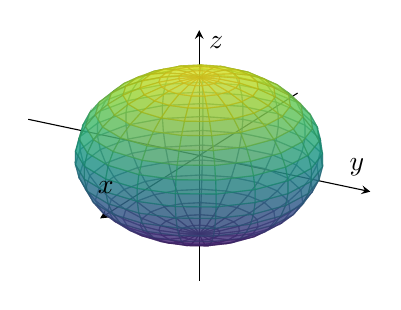
\begin{tikzpicture}[scale=1.0]
    \begin{axis}[
        view={120}{30},
        axis lines=center,
        xlabel=$x$, ylabel=$y$, zlabel=$z$,
        ticks=none,
        enlargelimits=0.3,
        ]
        % Ellipsoid with a=2, b=1.5, c=1
        \addplot3[
            surf,
            domain=0:360,
            y domain=0:180,
            samples=20,
            opacity=0.6,
            colormap/viridis,
        ]
        ({2*sin(y)*cos(x)}, {1.5*sin(y)*sin(x)}, {cos(y)});
    \end{axis}
\end{tikzpicture}
\captionof{figure}{Ellipsoid: $\frac{x^2}{4} + \frac{y^2}{2.25} + z^2 = 1$}
\end{center}

\Note[Cone]{
    The general equation of a cone that opens along the $z$-axis is \[ 
        \frac{(x-h)^2}{a^2} + \frac{(y-k)^2}{b^2} = \frac{(z-l)^2}{c^2}
    \]
    where $(h,k,l)$ is the center of the cone and $a, b, c$ are the semi-axis lengths. \\
}

\begin{center}
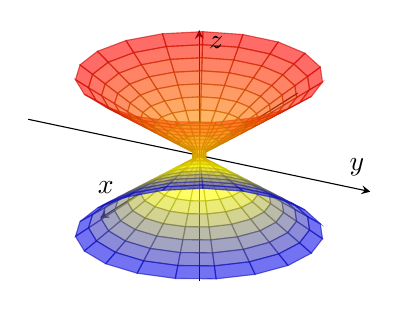
\begin{tikzpicture}[scale=1.0]
    \begin{axis}[
        view={120}{30},
        axis lines=center,
        xlabel=$x$, ylabel=$y$, zlabel=$z$,
        ticks=none,
        enlargelimits=0.3,
        zmin=-2, zmax=2,
        ]
        % Cone: x^2 + y^2 = z^2
        \addplot3[
            surf,
            domain=0:360,
            y domain=-2:2,
            samples=20,
            opacity=0.6,
            colormap/hot,
        ]
        ({abs(y)*cos(x)}, {abs(y)*sin(x)}, {y});
    \end{axis}
\end{tikzpicture}
\captionof{figure}{Cone: $x^2 + y^2 = z^2$}
\end{center}

\Note[Cylinder]{
    The general equation of a cylinder that opens along the $z$-axis is \[ 
        \frac{(x-h)^2}{a^2} + \frac{(y-k)^2}{b^2} = 1
    \]
    where $(h,k)$ is the center of the cylinder and $a, b$ are the semi-axis lengths. \\
    If $a = b$, we get a circular cylinder.
}

\begin{center}
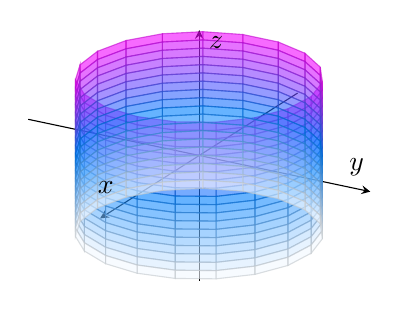
\begin{tikzpicture}[scale=1.0]
    \begin{axis}[
        view={120}{30},
        axis lines=center,
        xlabel=$x$, ylabel=$y$, zlabel=$z$,
        ticks=none,
        enlargelimits=0.3,
        zmin=-2, zmax=2,
        ]
        % Cylinder: x^2 + y^2 = 1
        \addplot3[
            surf,
            domain=0:360,
            y domain=-2:2,
            samples=20,
            opacity=0.6,
            colormap/cool,
        ]
        ({cos(x)}, {sin(x)}, {y});
    \end{axis}
\end{tikzpicture}
\captionof{figure}{Circular Cylinder: $x^2 + y^2 = 1$}
\end{center}

\Note[Hyperboloid of One Sheet]{
    The general equation of a hyperboloid of one sheet is \[ 
        \frac{(x-h)^2}{a^2} + \frac{(y-k)^2}{b^2} - \frac{(z-l)^2}{c^2} = 1
    \]
    where $(h,k,l)$ is the center of the hyperboloid and $a, b, c$ are the semi-axis lengths. \\
}

\begin{center}
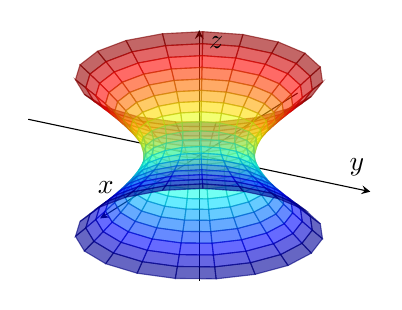
\begin{tikzpicture}[scale=1.0]
    \begin{axis}[
        view={120}{30},
        axis lines=center,
        xlabel=$x$, ylabel=$y$, zlabel=$z$,
        ticks=none,
        enlargelimits=0.3,
        zmin=-2, zmax=2,
        ]
        % Hyperboloid of one sheet: x^2 + y^2 - z^2 = 1
        \addplot3[
            surf,
            domain=0:360,
            y domain=-2:2,
            samples=20,
            opacity=0.6,
            colormap/jet,
        ]
        ({sqrt(1+y*y)*cos(x)}, {sqrt(1+y*y)*sin(x)}, {y});
    \end{axis}
\end{tikzpicture}
\captionof{figure}{Hyperboloid of One Sheet: $x^2 + y^2 - z^2 = 1$}
\end{center}

\Note[Hyperboloid of Two Sheets]{
    The general equation of a hyperboloid of two sheets is \[ 
        -\frac{(x-h)^2}{a^2} - \frac{(y-k)^2}{b^2} + \frac{(z-l)^2}{c^2} = 1
    \]
    where $(h,k,l)$ is the center of the hyperboloid and $a, b, c$ are the semi-axis lengths. \\
}

\begin{center}
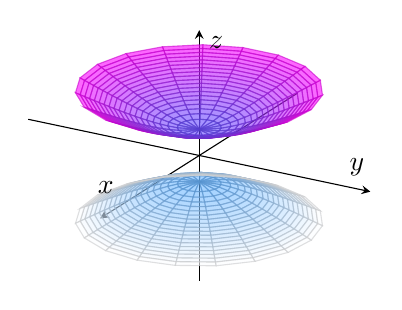
\begin{tikzpicture}[scale=1.0]
    \begin{axis}[
        view={120}{30},
        axis lines=center,
        xlabel=$x$, ylabel=$y$, zlabel=$z$,
        ticks=none,
        enlargelimits=0.3,
        zmin=-3, zmax=3,
        ]
        % Hyperboloid of two sheets: z^2 - x^2 - y^2 = 1
        % Upper sheet
        \addplot3[
            surf,
            domain=0:360,
            y domain=1:2.5,
            samples=20,
            opacity=0.6,
            colormap/cool,
        ]
        ({sqrt(y*y-1)*cos(x)}, {sqrt(y*y-1)*sin(x)}, {y});
        % Lower sheet
        \addplot3[
            surf,
            domain=0:360,
            y domain=-2.5:-1,
            samples=20,
            opacity=0.6,
            colormap/cool,
        ]
        ({sqrt(y*y-1)*cos(x)}, {sqrt(y*y-1)*sin(x)}, {y});
    \end{axis}
\end{tikzpicture}
\captionof{figure}{Hyperboloid of Two Sheets: $z^2 - x^2 - y^2 = 1$}
\end{center}

\Note[Elliptic Paraboloid]{
    The general equation of an elliptic paraboloid is \[ 
        \frac{(x-h)^2}{a^2} + \frac{(y-k)^2}{b^2} = \frac{z-l}{c}
    \]
    where $(h,k,l)$ is the center of the paraboloid and $a, b$ are the semi-axis lengths. \\
}

\begin{center}
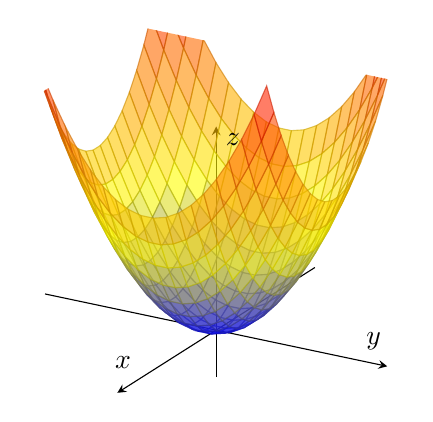
\begin{tikzpicture}[scale=1.0]
    \begin{axis}[
        view={120}{30},
        axis lines=center,
        xlabel=$x$, ylabel=$y$, zlabel=$z$,
        ticks=none,
        enlargelimits=0.3,
        zmin=0, zmax=4,
        ]
        % Elliptic paraboloid: z = x^2 + y^2
        \addplot3[
            surf,
            domain=-2:2,
            y domain=-2:2,
            samples=20,
            opacity=0.6,
            colormap/hot,
        ]
        ({x}, {y}, {x*x + y*y});
    \end{axis}
\end{tikzpicture}
\captionof{figure}{Elliptic Paraboloid: $z = x^2 + y^2$}
\end{center}

\Note[Hyperbolic Paraboloid]{
    The general equation of a hyperbolic paraboloid is \[ 
        \frac{(x-h)^2}{a^2} - \frac{(y-k)^2}{b^2} = \frac{z-l}{c}
    \]
    where $(h,k,l)$ is the center of the paraboloid and $a, b$ are the semi-axis lengths. \\
}

\begin{center}
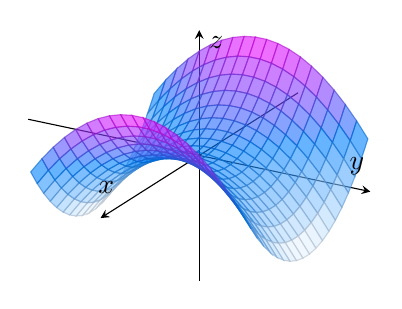
\begin{tikzpicture}[scale=1.0]
    \begin{axis}[
        view={120}{30},
        axis lines=center,
        xlabel=$x$, ylabel=$y$, zlabel=$z$,
        ticks=none,
        enlargelimits=0.3,
        zmin=-4, zmax=4,
        ]
        % Hyperbolic paraboloid (saddle): z = x^2 - y^2
        \addplot3[
            surf,
            domain=-2:2,
            y domain=-2:2,
            samples=20,
            opacity=0.6,
            colormap/cool,
        ]
        ({x}, {y}, {x*x - y*y});
    \end{axis}
\end{tikzpicture}
\captionof{figure}{Hyperbolic Paraboloid (Saddle): $z = x^2 - y^2$}
\end{center}


%%%%%%%%%%%%%%%%%%%%%%%%%%%%%%%%%%%%
%  Calculus with Vector Functions  %
%%%%%%%%%%%%%%%%%%%%%%%%%%%%%%%%%%%%

\subsection{Calculus with Vector Functions}

Let \[
    \vec{r}(t) = \langle f(t), g(t), h(t) \rangle
\]

\Note{
    \[ \lim_{t \to a} \vec{r}(t) = \langle \lim_{t \to a} f(t), \lim_{t \to a} g(t), \lim_{t \to a} h(t) \rangle \]
}

\Note{
    \[ \dv{}{t} \left(\vec{u} + \vec{v}\right) = \vec{u}' + \vec{v}'  \]
    \[ \dv{}{t} \left(c\vec{u}\right) = c\vec{u}' \]
    \[ \dv{}{t} \left(\vec{u} \cdot \vec{v}\right) = \vec{u}' \cdot \vec{v} + \vec{u} \cdot \vec{v}'  \]
    \[ \dv{}{t} \left(\vec{u} \times \vec{v}\right) = \vec{u}' \times \vec{v} + \vec{u} \times \vec{v}'  \]
    \[ \dv{}{t} \left( \vec{u}f(t) \right) = f'(t)\vec{u}'(f(t))  \]
}

\Note{
    \[ \int \vec{r}(t) \dd{t} = \langle \int f(t) \dd{t}, \int g(t) \dd{t}, \int h(t) \dd{t} \rangle \]
    \[ \int_{a}^{b} \vec{r}(t) \dd{t} = \Biggl\langle \int_{a}^{b} f(t) \dd{t} + \int_{a}^{b} g(t) \dd{t} + \int_{a}^{b} h(t) \dd{t} \Biggr\rangle \]
}


%%%%%%%%%%%%%%%%%%%%%%%%%%%%%%%%%%%%%%%%%%%
%  Tangent, Normal, and Binormal Vectors  %
%%%%%%%%%%%%%%%%%%%%%%%%%%%%%%%%%%%%%%%%%%%

\subsection{Tangent, Normal, and Binormal Vectors}

\Note[Unit Tangent vector]{
    Given the vector function $\vec{r}(t)$, we call $\vec{r}'(t)$ the \textbf{tangent vector}
    The unit tangent vector is given by \[ 
        \vec{T}(t) = \frac{\vec{r}'(t)}{\lVert \vec{r}'(t) \rVert}
    \]
}

\Note[Unit Normal vector]{
    If $\vec{T}(t)$ is the unit tangent vector, then the \textbf{unit normal vector} is given by \[ 
        \vec{N}(t) = \frac{\vec{T}'(t)}{\lVert \vec{T}'(t) \rVert}
    \]
}

\Note{
    If $\vec{r}(t)$ is a vector such that $\lVert \vec{r}(t) \rVert = c$ for all $t$, then $\vec{r}'(t)$ is orthogonal to $\vec{r}(t)$
}

\Note[Binormal vector]{
    The \textbf{binormal vector} is given by \[ 
        \vec{B}(t) = \vec{T}(t) \times \vec{N}(t)
    \]
    The binormal vector is orthogonal to both the tangent and normal vectors.
}

\begin{center}
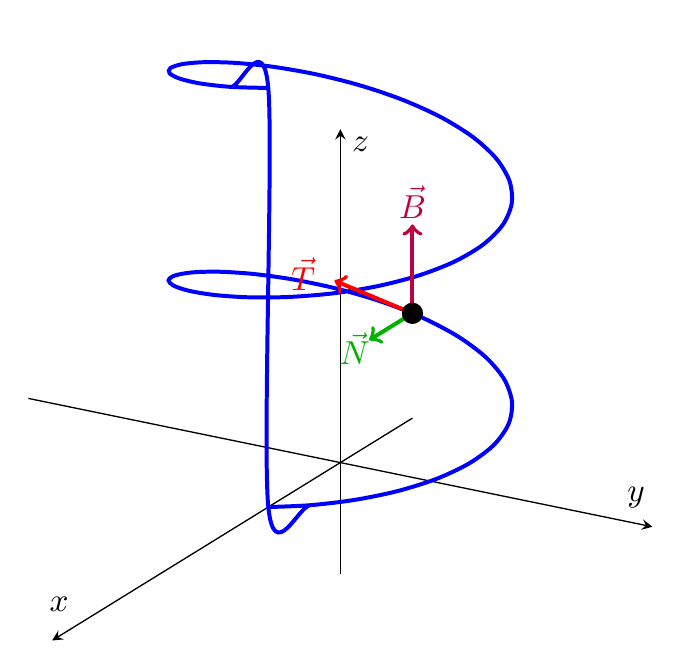
\begin{tikzpicture}[scale=1.2]
    \begin{axis}[
        view={120}{30},
        axis lines=center,
        xlabel=$x$, ylabel=$y$, zlabel=$z$,
        xmin=-1, xmax=4,
        ymin=-2, ymax=2,
        zmin=-1, zmax=3,
        ticks=none,
        width=12cm, height=10cm,
        ]
        % Helix curve
        \addplot3[blue, very thick, domain=0:4*pi, samples=50, smooth]
            ({cos(deg(x))}, {sin(deg(x))}, {0.3*x});
        
        % Point on curve at t=pi
        \addplot3[mark=*, mark size=3pt, black] coordinates {({cos(180)}, {sin(180)}, {0.3*pi})};
        
        % Tangent vector (red)
        \draw[->, red, very thick] ({cos(180)}, {sin(180)}, {0.3*pi}) -- 
            ({cos(180)-0.5*sin(180)}, {sin(180)+0.5*cos(180)}, {0.3*pi+0.15});
        \node[red] at ({cos(180)-0.7*sin(180)}, {sin(180)+0.7*cos(180)}, {0.3*pi+0.15}) {$\vec{T}$};
        
        % Normal vector (green)
        \draw[->, green!70!black, very thick] ({cos(180)}, {sin(180)}, {0.3*pi}) -- 
            ({cos(180)-0.6*cos(180)}, {sin(180)-0.6*sin(180)}, {0.3*pi});
        \node[green!70!black] at ({cos(180)-0.8*cos(180)}, {sin(180)-0.8*sin(180)}, {0.3*pi}) {$\vec{N}$};
        
        % Binormal vector (purple)
        \draw[->, purple, very thick] ({cos(180)}, {sin(180)}, {0.3*pi}) -- 
            ({cos(180)}, {sin(180)}, {0.3*pi+0.8});
        \node[purple] at ({cos(180)}, {sin(180)}, {0.3*pi+1}) {$\vec{B}$};
    \end{axis}
\end{tikzpicture}
\captionof{figure}{TNB Frame (Frenet-Serret Frame) on a helix $\vec{r}(t) = \langle \cos t, \sin t, 0.3t \rangle$}
\end{center}


%%%%%%%%%%%%%%%%%%%%%%%%%%%%%%%%%%%%%%
%  Arc Length with Vector Functions  %
%%%%%%%%%%%%%%%%%%%%%%%%%%%%%%%%%%%%%%

\subsection{Arc Length with Vector Functions}

\Note{
    The arc length of a vector function $\vec{r}(t)$ from $t=a$ to $t=b$ is given by \[ 
        L = \int_{a}^{b} \lVert \vec{r}'(t) \rVert \dd{t}
    \]
    Or, \[
        L = \int_{a}^{b} \sqrt{\left( \dv{f}{t} \right)^2 + \left( \dv{g}{t} \right)^2 + \left( \dv{h}{t} \right)^2} \dd{t}
    \]
}


%%%%%%%%%%%%%%%
%  Curvature  %
%%%%%%%%%%%%%%%

\subsection{Curvature}

\Note[Curvature of a curve in 3-D space]{
    The curvature of a curve in 3-D space is given by \[ 
        \kappa = \frac{\lVert \vec{T}'(t) \rVert}{\lVert \vec{r}'(t) \rVert}
    \]
    where $\vec{T}(t)$ is the unit tangent vector and $\vec{r}(t)$ is the position vector. \\
    This can also be written as \[ 
        \kappa = \frac{\lVert \vec{r}'(t) \times \vec{r}''(t) \rVert}{\lVert \vec{r}'(t) \rVert^3}
    \]
}
